\documentclass[9.5pt]{article}
\usepackage{geometry}
\geometry{a4paper, margin=1in}
\usepackage{graphicx}
\usepackage{amsmath, amssymb}
\usepackage{setspace}
\usepackage{titlesec}
\usepackage{fancyhdr}
\usepackage{hyperref}
\usepackage{listings}
\usepackage{xcolor}
\usepackage{enumitem}
\usepackage{fontspec}
\usepackage{subcaption}
\usepackage{tabularx}
\setmainfont{Times New Roman}

\titleformat{\section}{\large\bfseries}{\thesection.}{1em}{}
\titleformat{\subsection}{\normalsize\bfseries}{\thesubsection.}{1em}{}

\pagestyle{fancy}
\fancyhf{}
\rhead{Luna Sugiyama}
\lhead{Final Report: Wed2 Natural Language Processing}
\rfoot{\thepage}

\title{\textbf{Evaluation of Claude Code and Gemini CLI}}
% \vspace{0.5em}
% \large [Optional Subtitle]}
\author{
    \makebox[\textwidth][c]{\textbf{Luna Sugiyama}} \\
    \makebox[\textwidth][c]{Information and Communication Engineering} \\
    \makebox[\textwidth][c]{\texttt{lunagracesugiyama@g.ecc.u-tokyo.ac.jp}}
}
\date{\today}

\begin{document}

\maketitle
\thispagestyle{fancy}
I have recently been interested in AI assistant tools to help software development~\cite{vibecoding}.
However, due to the pricing I have not been able to use them extensively.
I thought this would be a good opportunity to explore these tools.
In this report I will choose these services and evaluate them on various tasks and aspects to see their strengths and weaknesses.

\section{About Each Service}
\subsection{Claude Code}
Claude Code is a code-centric variant of the Claude family of AI models developed by Anthropic. It is optimized for software development and programming-related tasks, such as code generation, debugging, explanation, and refactoring~\cite{anthropic_claudecode}.
\subsection{Gemini CLI}
Gemini CLI is an open-source AI agent by Google that brings Gemini into the terminal and supports code editing, task management, research integration via web search, and tooling like Imagen and Veo~\cite{google_gemini_cli}.

\section{Tasks}
\subsection{Task 1: Code Generation}
The task for code generation is:
\begin{verbatim}
    Build a responsive map of a shop with several floors and can search which product is where.
\end{verbatim}
\subsubsection{Claude Code}
I was only asked once whether I want to create a index.html and made the rest automatically\footnote{Generated files can be found at \url{https://github.com/LunaSugiyama/masters/tree/main/wed2llm/claude_generation}.}
The method used for searching products was simple string matching.
The generated files include index.html, style.css, app.js, data.js, and a README.md file.

\subsubsection{Gemini CLI}
I was asked whether gemini could use npx, mkdir and other commands\footnote{Generated files can be found at \url{https://github.com/LunaSugiyama/masters/tree/main/wed2llm/gemini_generation/shop-map}.}
I was not asked this question in Claude Code so perhaps Gemini CLI is more cautious about executing commands.
The time for generation was about 15 minutes.
However, when running the generated code, it just started the default React app page.
Therefore, I had to ask Gemini CLI to fix the code.
Moreover, an error existed in the JSON code for the products, which was simple but had to be fixed.

\subsubsection{Comparison}
\begin{table}[h]
\centering
\caption{Comparison of Claude Code and Gemini CLI for Code Generation Task}
\label{tab:code_generation_comparison}
\renewcommand{\arraystretch}{1.2}
\begin{tabularx}{\textwidth}{|X|X|X|}
\hline
\textbf{Criteria} & \textbf{Claude Code} & \textbf{Gemini CLI} \\
\hline
Command Caution & Did not ask about permission to run commands & Asked whether it could run `npx`, `mkdir`, etc. \\
\hline
Response Speed & Fast (under 5 min) & Slow (about 15 minutes) \\
\hline
File Generation & Automatically generated `index.html`, `style.css`, `app.js`, `data.js`, and `README.md` & Generated initial React project but required 'App.js' and JSON correction \\
\hline
Search Logic & Used simple string matching over all floor data & Similar string matching, but only applied to the current floor \\
\hline
Execution Outcome & Simple working web app with working search feature & React page; minimum page with no map-like component \\
\hline
Error Presence & No errors in generated code & JSON error and missing configuration in app setup \\
\hline
Overall Score & High & Moderate \\
\hline
\end{tabularx}
\end{table}

\subsection{Task 2: Repository Code Explanation}
The task for code explanation is:
\begin{verbatim}
the repository pytorch has implementation loss.backward can you explain how this is implemented and what it does in detail?
\end{verbatim}
\subsubsection{Claude Code}
The Todos that Claude Code generated for this task can be found in Appendix~\ref{sec:code_explanation_output}.
I asked additional question what grad\_fn.backward does and asked it to save the output to a file.
Here is the link to the file generated by Claude Code: \url{https://github.com/LunaSugiyama/masters/blob/main/wed2llm/explanation_task/claude_pytorch_loss_backward_explanation.md}.

\subsubsection{Gemini CLI}
The Todos that Gemini CLI generated for this task can be found in Appendix~\ref{sec:code_explanation_output}.
No additional questions were asked because the output was satisfactory.
Here is the link to the file generated by Gemini CLI: \url{https://github.com/LunaSugiyama/masters/blob/main/wed2llm/explanation_task/gemini_pytorch_loss_backward_explanation.md}.
\subsection{Comparison}
It is summarized in Table~\ref{tab:code_explanation_comparison}.
\begin{table}[htp]
\centering
\caption{Comparison of Claude Code and Gemini CLI on Code Explanation Task}
\label{tab:code_explanation_comparison}
\renewcommand{\arraystretch}{1.2}
\begin{tabularx}{\textwidth}{|X|X|X|}
\hline
\textbf{Criteria} & \textbf{Claude Code Output} & \textbf{Gemini CLI Output} \\
\hline
\textbf{Clarity of Explanation} & Provides a clear, structured explanation in natural language & Also clear, with additional context about autograd and computational graph \\
\hline
\textbf{Technical Depth} & High: explains gradients, tensors, and autograd in PyTorch & High: mentions backward pass, dynamic computation graph, and gradient accumulation \\
\hline
\textbf{Step-by-step Breakdown} & Yes: explains what happens internally when `loss.backward()` is called & Yes: walks through how gradients are computed and stored \\
\hline
\textbf{Use of Terminology} & Uses terms like gradient, autograd, tensor, computation graph & Uses same terms but also mentions `leaf tensor`, `requires\_grad`, and internal caching \\
\hline
\textbf{Code References} & Does not reference surrounding code explicitly & Includes helpful mention of `loss = criterion(output, target)` context \\
\hline
\textbf{Extra Insights} & Notes about default behavior of `.backward()` and single scalar gradients & Mentions that `.backward()` works only when the tensor is scalar, else `grad` arg is required \\
\hline
\textbf{Overall Usefulness} & Very useful for intermediate-level users, need extra question for deep understanding & Slightly more comprehensive, especially for users unfamiliar with autograd \\
\hline
\end{tabularx}
\end{table}

\subsection{Task 3: Code Review}
The task for code review is to review the following code (code developed in a hackathon with a duration of 3 days) and suggest improvements \url{https://github.com/asahi1199/mobility-adventure}:
\begin{verbatim}
    "could you review the codes in this repository and make it more clear and clean"
\end{verbatim}
\subsubsection{Claude Code}
It tooks about 3 minutes to generate the review.
The issues that Claude Code found were:
\begin{enumerate}
    \item Inconsistent naming: DogCLASS should be Dog (interface/type names should be PascalCase)
    \item Poor variable naming: setid should be setId, idValue could be clearer
    \item Console.log statements left in production code
    \item Unused imports and variables
    \item Inconsistent component structure between pages
    \item Magic numbers and hardcoded values
    \item Large component (gesture\_component.tsx) needs refactoring
\end{enumerate}
After confirming to me that it is okay to fix the code, it fixed and asked whether it can run the code to test it.

\subsubsection{Gemini CLI}
It took about 1 minute to generate the review.
The issues that Gemini CLI found were:
\begin{enumerate}
    \item Rename \texttt{gesture\_component.tsx} to \texttt{InteractiveMap.tsx} and rename the component \texttt{CroppableImage} to \texttt{InteractiveMap}. This will better reflect the component's functionality.
    \item Refactor state management by grouping related state variables into objects.
    \item Create a custom hook \texttt{useDogs} to encapsulate the logic for managing both moving and stationary dogs. This will reduce code duplication and improve organization.
    \item Extract the drawer logic into a separate component. This will simplify the \texttt{InteractiveMap} component and make the code easier to understand.
    \item Remove hardcoded data. Fetch dog data from \texttt{dogdb.ts} and generate the initial positions dynamically.
    \item Improve comments and readability by adding more descriptive comments and using more meaningful variable names.
\end{enumerate}
After confirming to me that it is okay to fix the code, it fixed and asked whether it can run the code to test it.

\section{Comparison of Code Review}
It is summarized in Table~\ref{tab:code_review_comparison}.
\begin{table}[h]
\centering
\caption{Comparison of Claude Code and Gemini CLI on Code Review Task}
\label{tab:code_review_comparison}
\renewcommand{\arraystretch}{1.2}
\begin{tabular}{|p{4cm}|p{5.5cm}|p{5.5cm}|}
\hline
\textbf{Criteria} & \textbf{Claude Code Output} & \textbf{Gemini CLI Output} \\
\hline
\textbf{Structure and Formatting} & Suggested renaming of components and restructuring for clarity (e.g., \texttt{gesture\_component.tsx} to \texttt{InteractiveMap.tsx}) & Recommended code separation and simplification, but focused less on naming conventions \\
\hline
\textbf{State Management} & Advocated grouping related state variables into objects for better organization & Highlighted redundancy and suggested using a single state object for cleaner updates \\
\hline
\textbf{Reusability} & Proposed a custom hook (\texttt{useDogs}) to manage moving/stationary entities & Emphasized modularity but did not explicitly propose hooks \\
\hline
\textbf{Component Design} & Recommended extracting drawer logic to a separate component & Also advised component splitting, focusing on the UI logic \\
\hline
\textbf{Data Management} & Suggested replacing hardcoded data with dynamic loading from \texttt{dogdb.ts} & Similar suggestion to load external data but less specific on the source \\
\hline
\textbf{Comments and Readability} & Recommended meaningful variable names and more descriptive comments & Mentioned improving clarity, but with less emphasis on inline comments \\
\hline
\textbf{Testing} & Asked for permission to run the code to test changes, indicating a hands-on approach & Did not automatically run tests. \\
\hline
\textbf{Overall Tone} & Direct and structured feedback, highly specific in instructions & More general advice, with an encouraging tone for improvement \\
\hline
\end{tabular}
\end{table}

\section{Evaluation Summary}
In this evaluation, I tested two modern AI assistants, Claude Code and Gemini CLI, on three software engineering tasks: code generation, code explanation, and code review. Both models performed well, with Claude Code generally offering more structured and specific responses, while Gemini CLI excelled in providing broader context and user-friendly guidance. Each tool's strengths and weaknesses were documented and compared in tables across the three tasks.
All tasks were performed using real repositories or prompts involving dynamic project setups, and responses were collected, documented, and verified manually.

\section{Discussion}
In this report, I explored two AI tools—Claude Code and Gemini CLI—both of which I had never used before. From an NLP perspective, both tools demonstrate strong natural language understanding and generation capabilities, as they can interpret developer intent and respond with relevant, contextually rich answers.
Claude Code showed remarkable coherence in its code review suggestions, often using precise terminology (e.g., "PascalCase", "hardcoded values", "drawer component separation"). Its responses reflect a rule-based reasoning style often used in formal technical communication. This indicates a robust grounding in structured code semantics and possibly reinforcement learning on code review corpora.
Gemini CLI, on the other hand, emphasized exploratory behavior. It simulated steps such as searching the codebase or running commands like `npx`, and provided a more conversational explanation. This suggests it models interactions more dialogically, aligning with Google's emphasis on multimodal and agent-like LLM interfaces.
The key NLP components demonstrated include:
\begin{itemize}
    \item \textbf{Intent Detection:} Both tools successfully inferred task goals from minimal input.
    \item \textbf{Contextual Reasoning:} Gemini especially showed strength in contextual searches (e.g., identifying where "backward" appears in a codebase).
    \item \textbf{Content Generation:} Both generated long-form explanations with minimal hallucination, adhering to project-specific information.
    \item \textbf{Interaction Modeling:} Claude asked for permission to refactor or run code, suggesting alignment with cooperative multi-turn dialogue paradigms.
\end{itemize}
Overall, trying these tools helped me understand how NLP models interface with software development workflows. They go beyond simple text generation by deeply understanding code structure, user goals, and project context—highlighting the growing integration of NLP and software engineering.

\clearpage
\section*{Appendix}
\appendix
\section{Which AI and How I Used It}
In addition to Claude Code and Gemini CLI, I utilized ChatGPT (developed by OpenAI) throughout the writing of this report. Specifically, ChatGPT was employed in the following ways:
\begin{itemize}
    \item \textbf{LaTeX Assistance:} ChatGPT helped generate LaTeX-compatible code for formatting tables, figures, and section layouts. This ensured that the report maintained a consistent and professional structure. 
    \item \textbf{Comparison Tables:} For comparing the output of Claude Code and Gemini CLI, I provided ChatGPT with change files or raw markdown output from each tool. ChatGPT synthesized this data and produced comparison tables highlighting key differences in their behavior and performance. 
    \item \textbf{Text Refinement:} Some sections of the report were edited with the help of ChatGPT to improve clarity, tone, and grammatical accuracy.
\end{itemize}
ChatGPT served as a supplementary writing assistant to streamline formatting and aid in comparative analysis between the AI tools under evaluation.

\section{Code Generation Output Screenshots}
See Fig.~\ref{fig:claude_code_output} and Fig.~\ref{fig:gemini_code_output} for screenshots of the code generation outputs from Claude Code and Gemini CLI, respectively.
\begin{figure}[htp]
    \centering
    \begin{subcaptionbox}[0.2\textwidth]{Claude Code CLI\label{fig:claude_cli}}
        {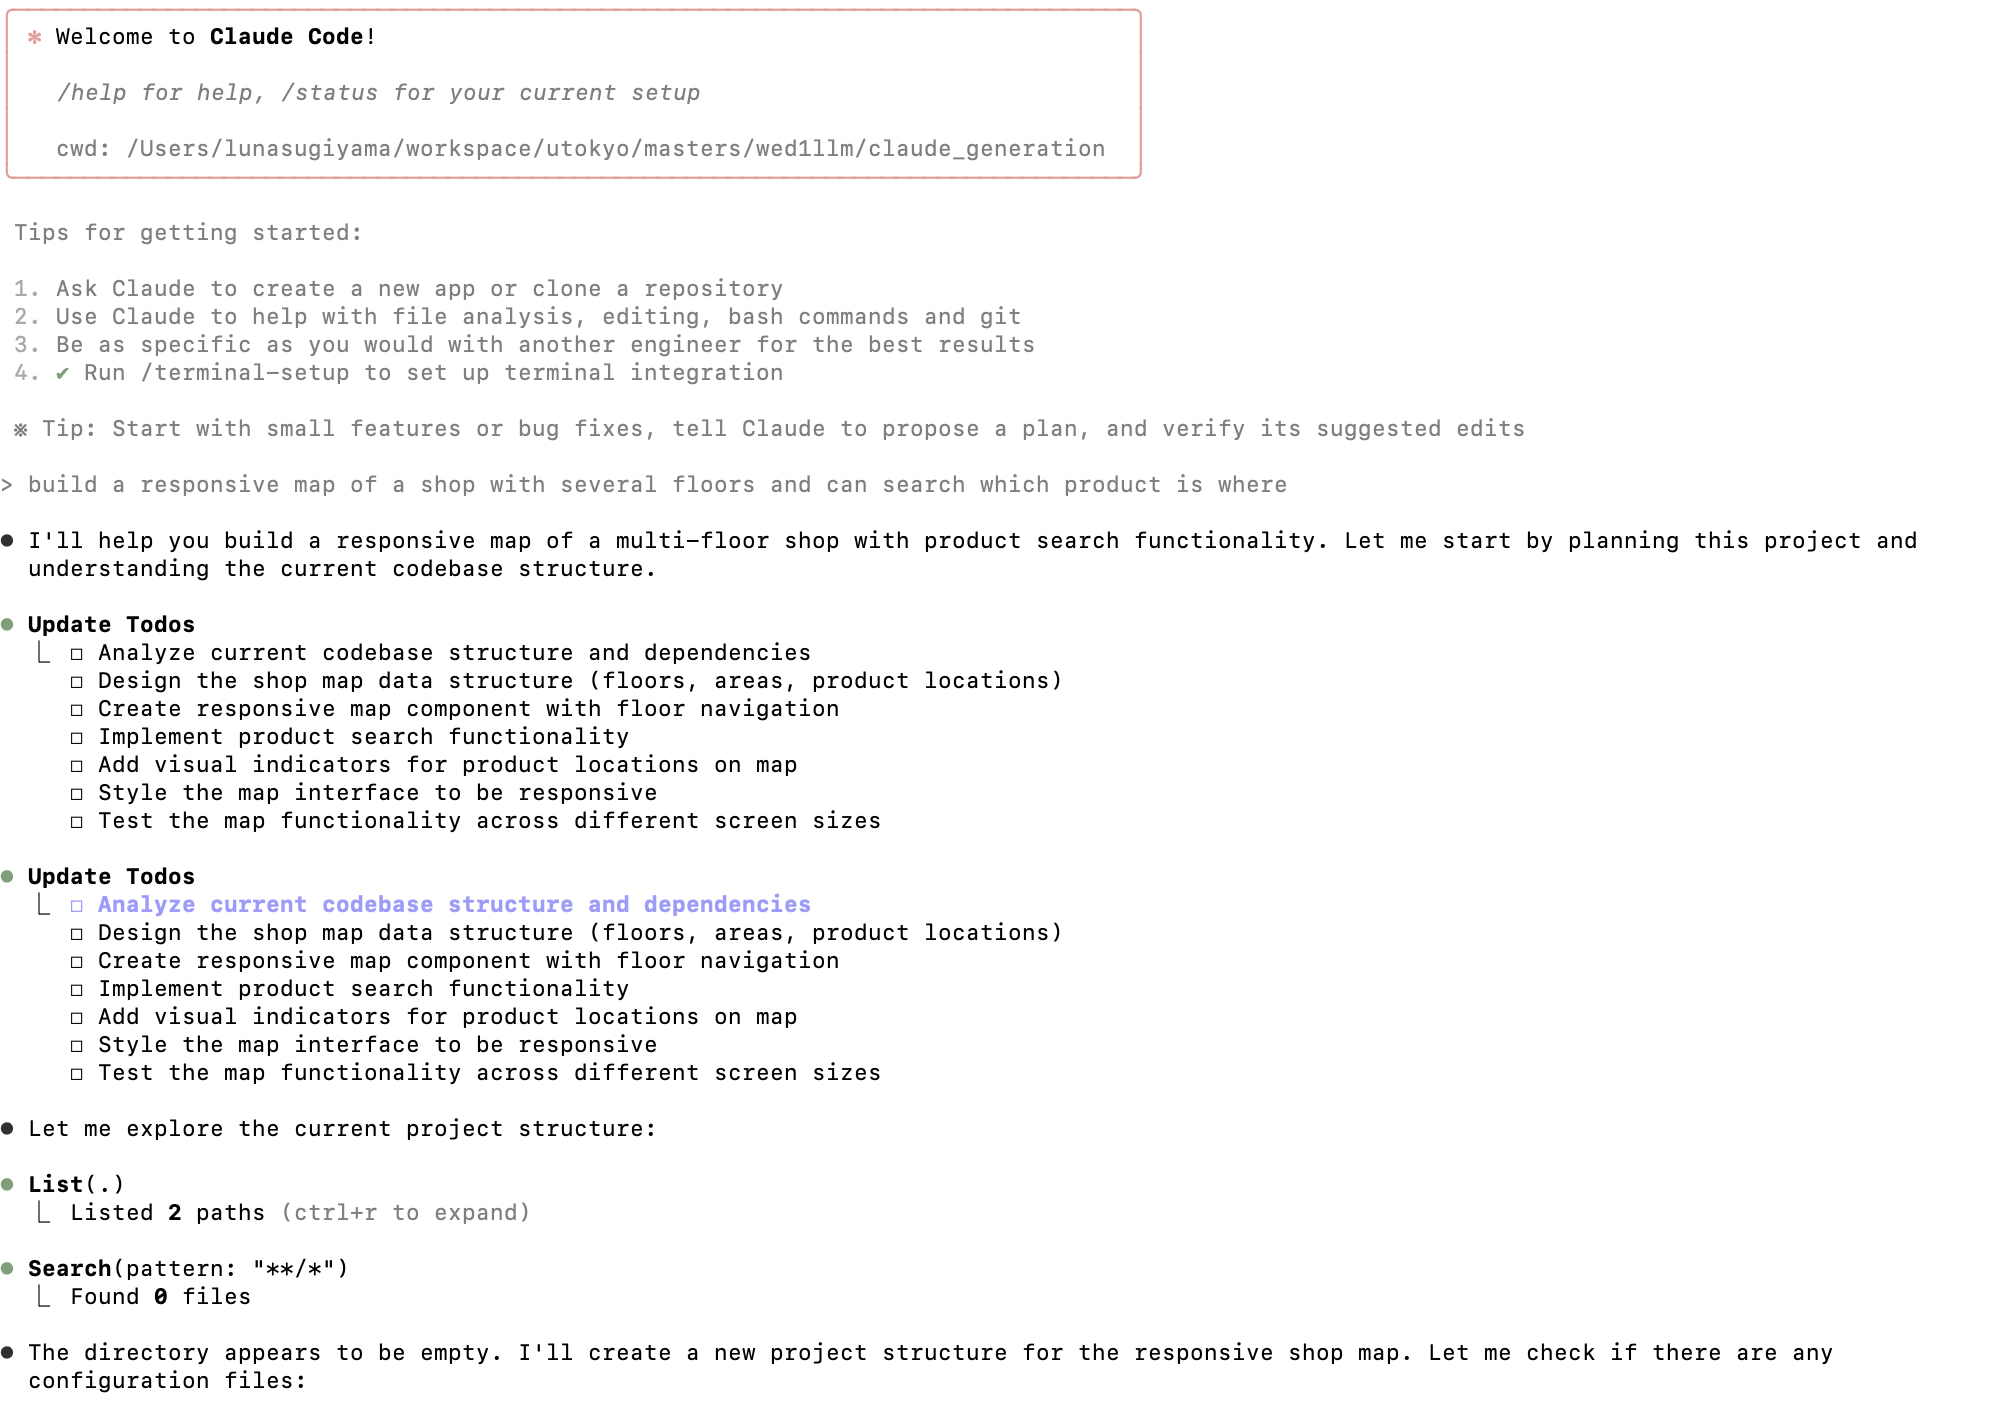
\includegraphics[width=0.7\linewidth]{figures/claude_cg_instruction.png}}
    \end{subcaptionbox}
    \hfill
    \begin{subcaptionbox}[0.2\textwidth]{Claude Code Generation Output\label{fig:claude_cg_output}}
        {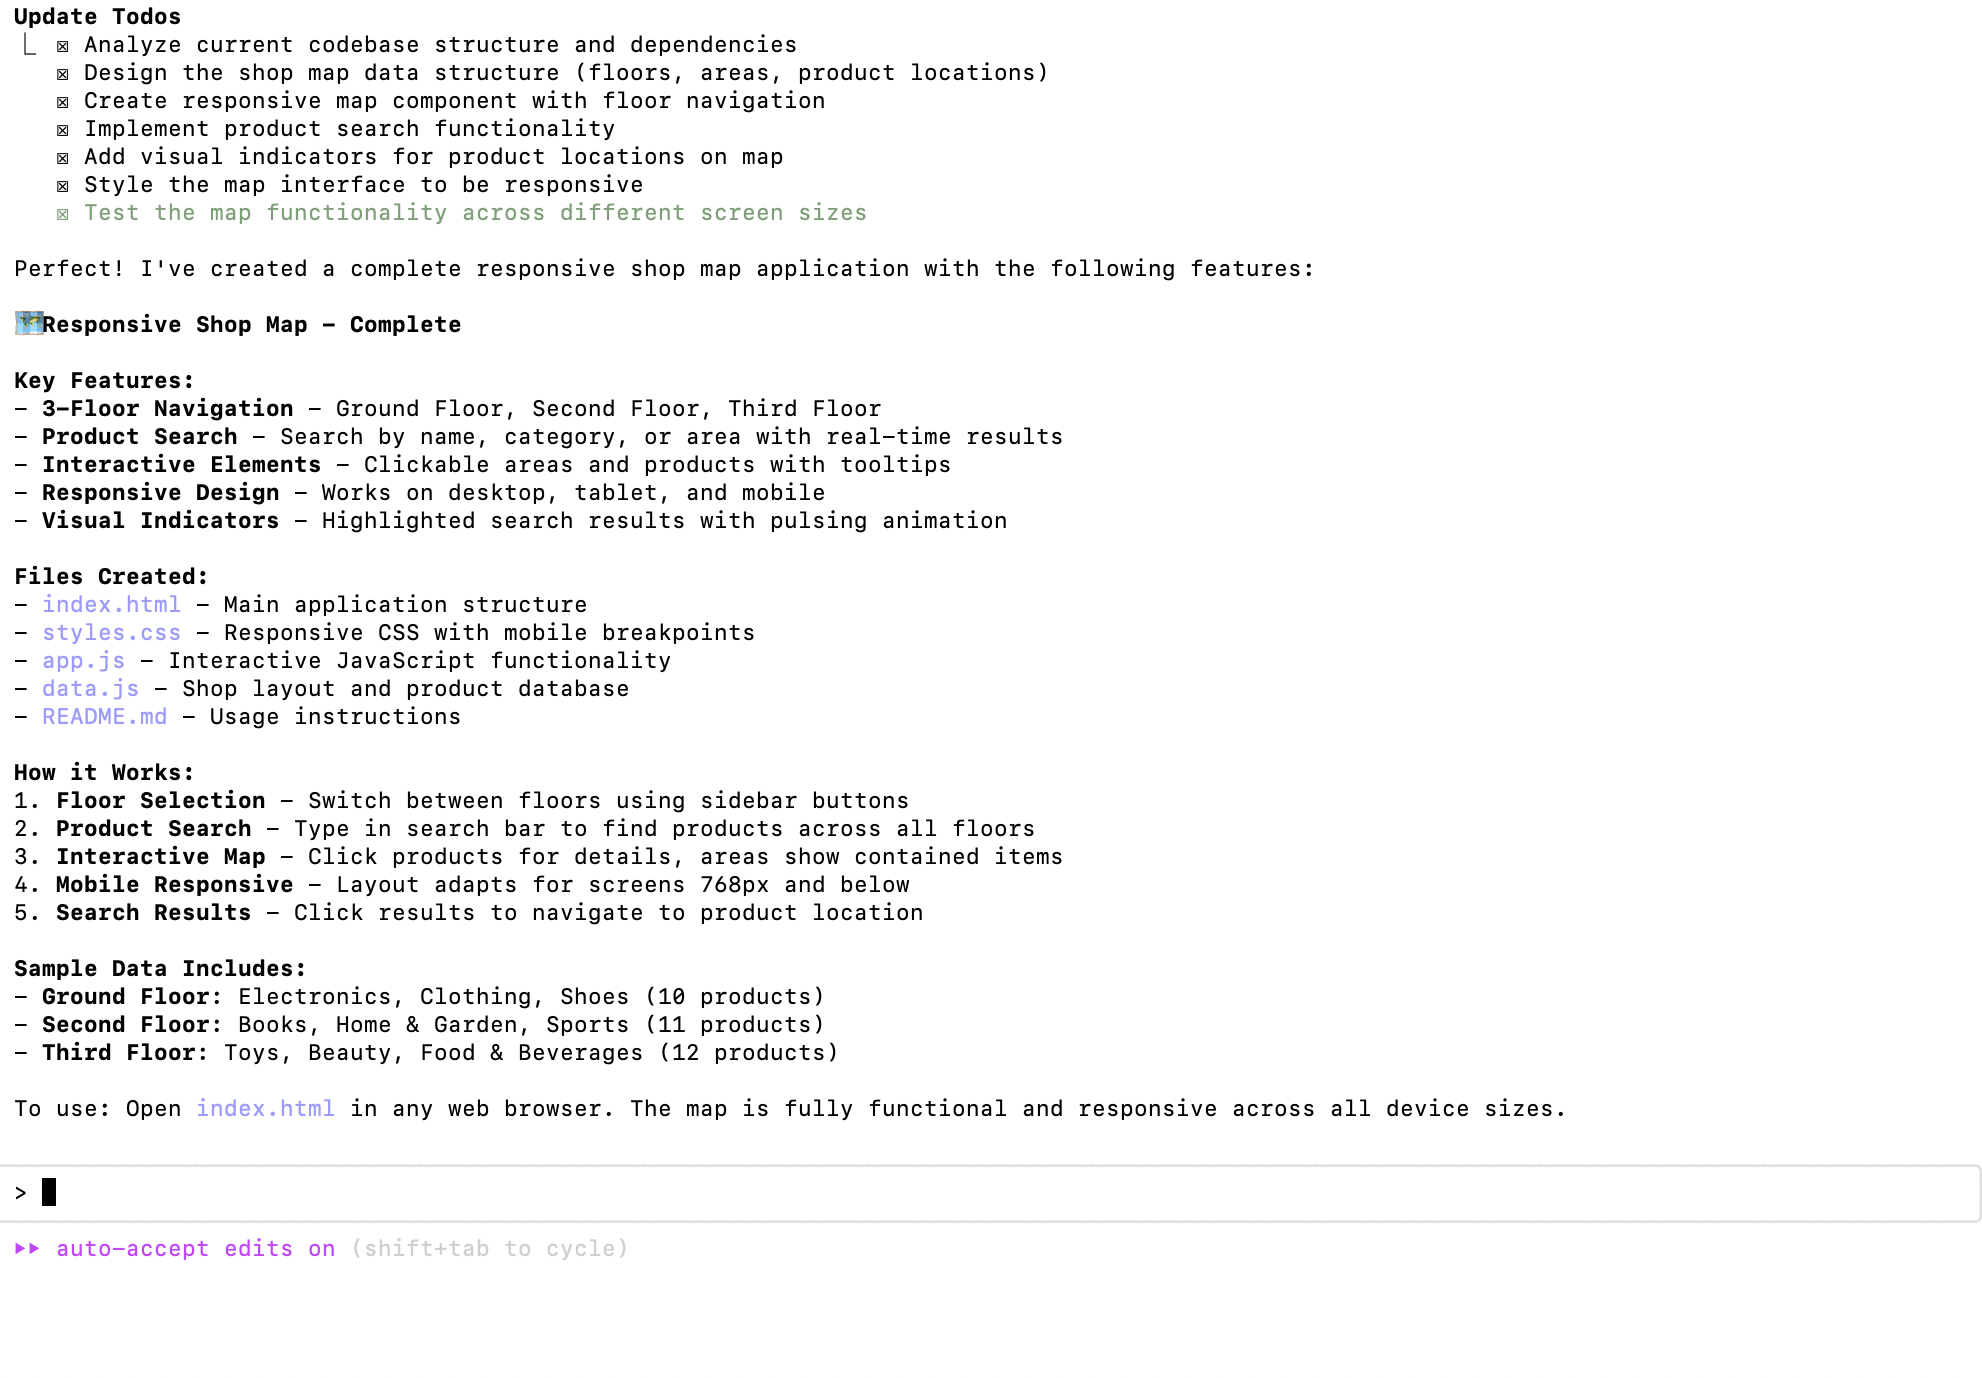
\includegraphics[width=0.7\linewidth]{figures/claude_cg_output.png}}
    \end{subcaptionbox}
    \hfill
    \begin{subcaptionbox}[0.2\textwidth]{Claude Code Generation Webpage\label{fig:claude_cg_web}}
        {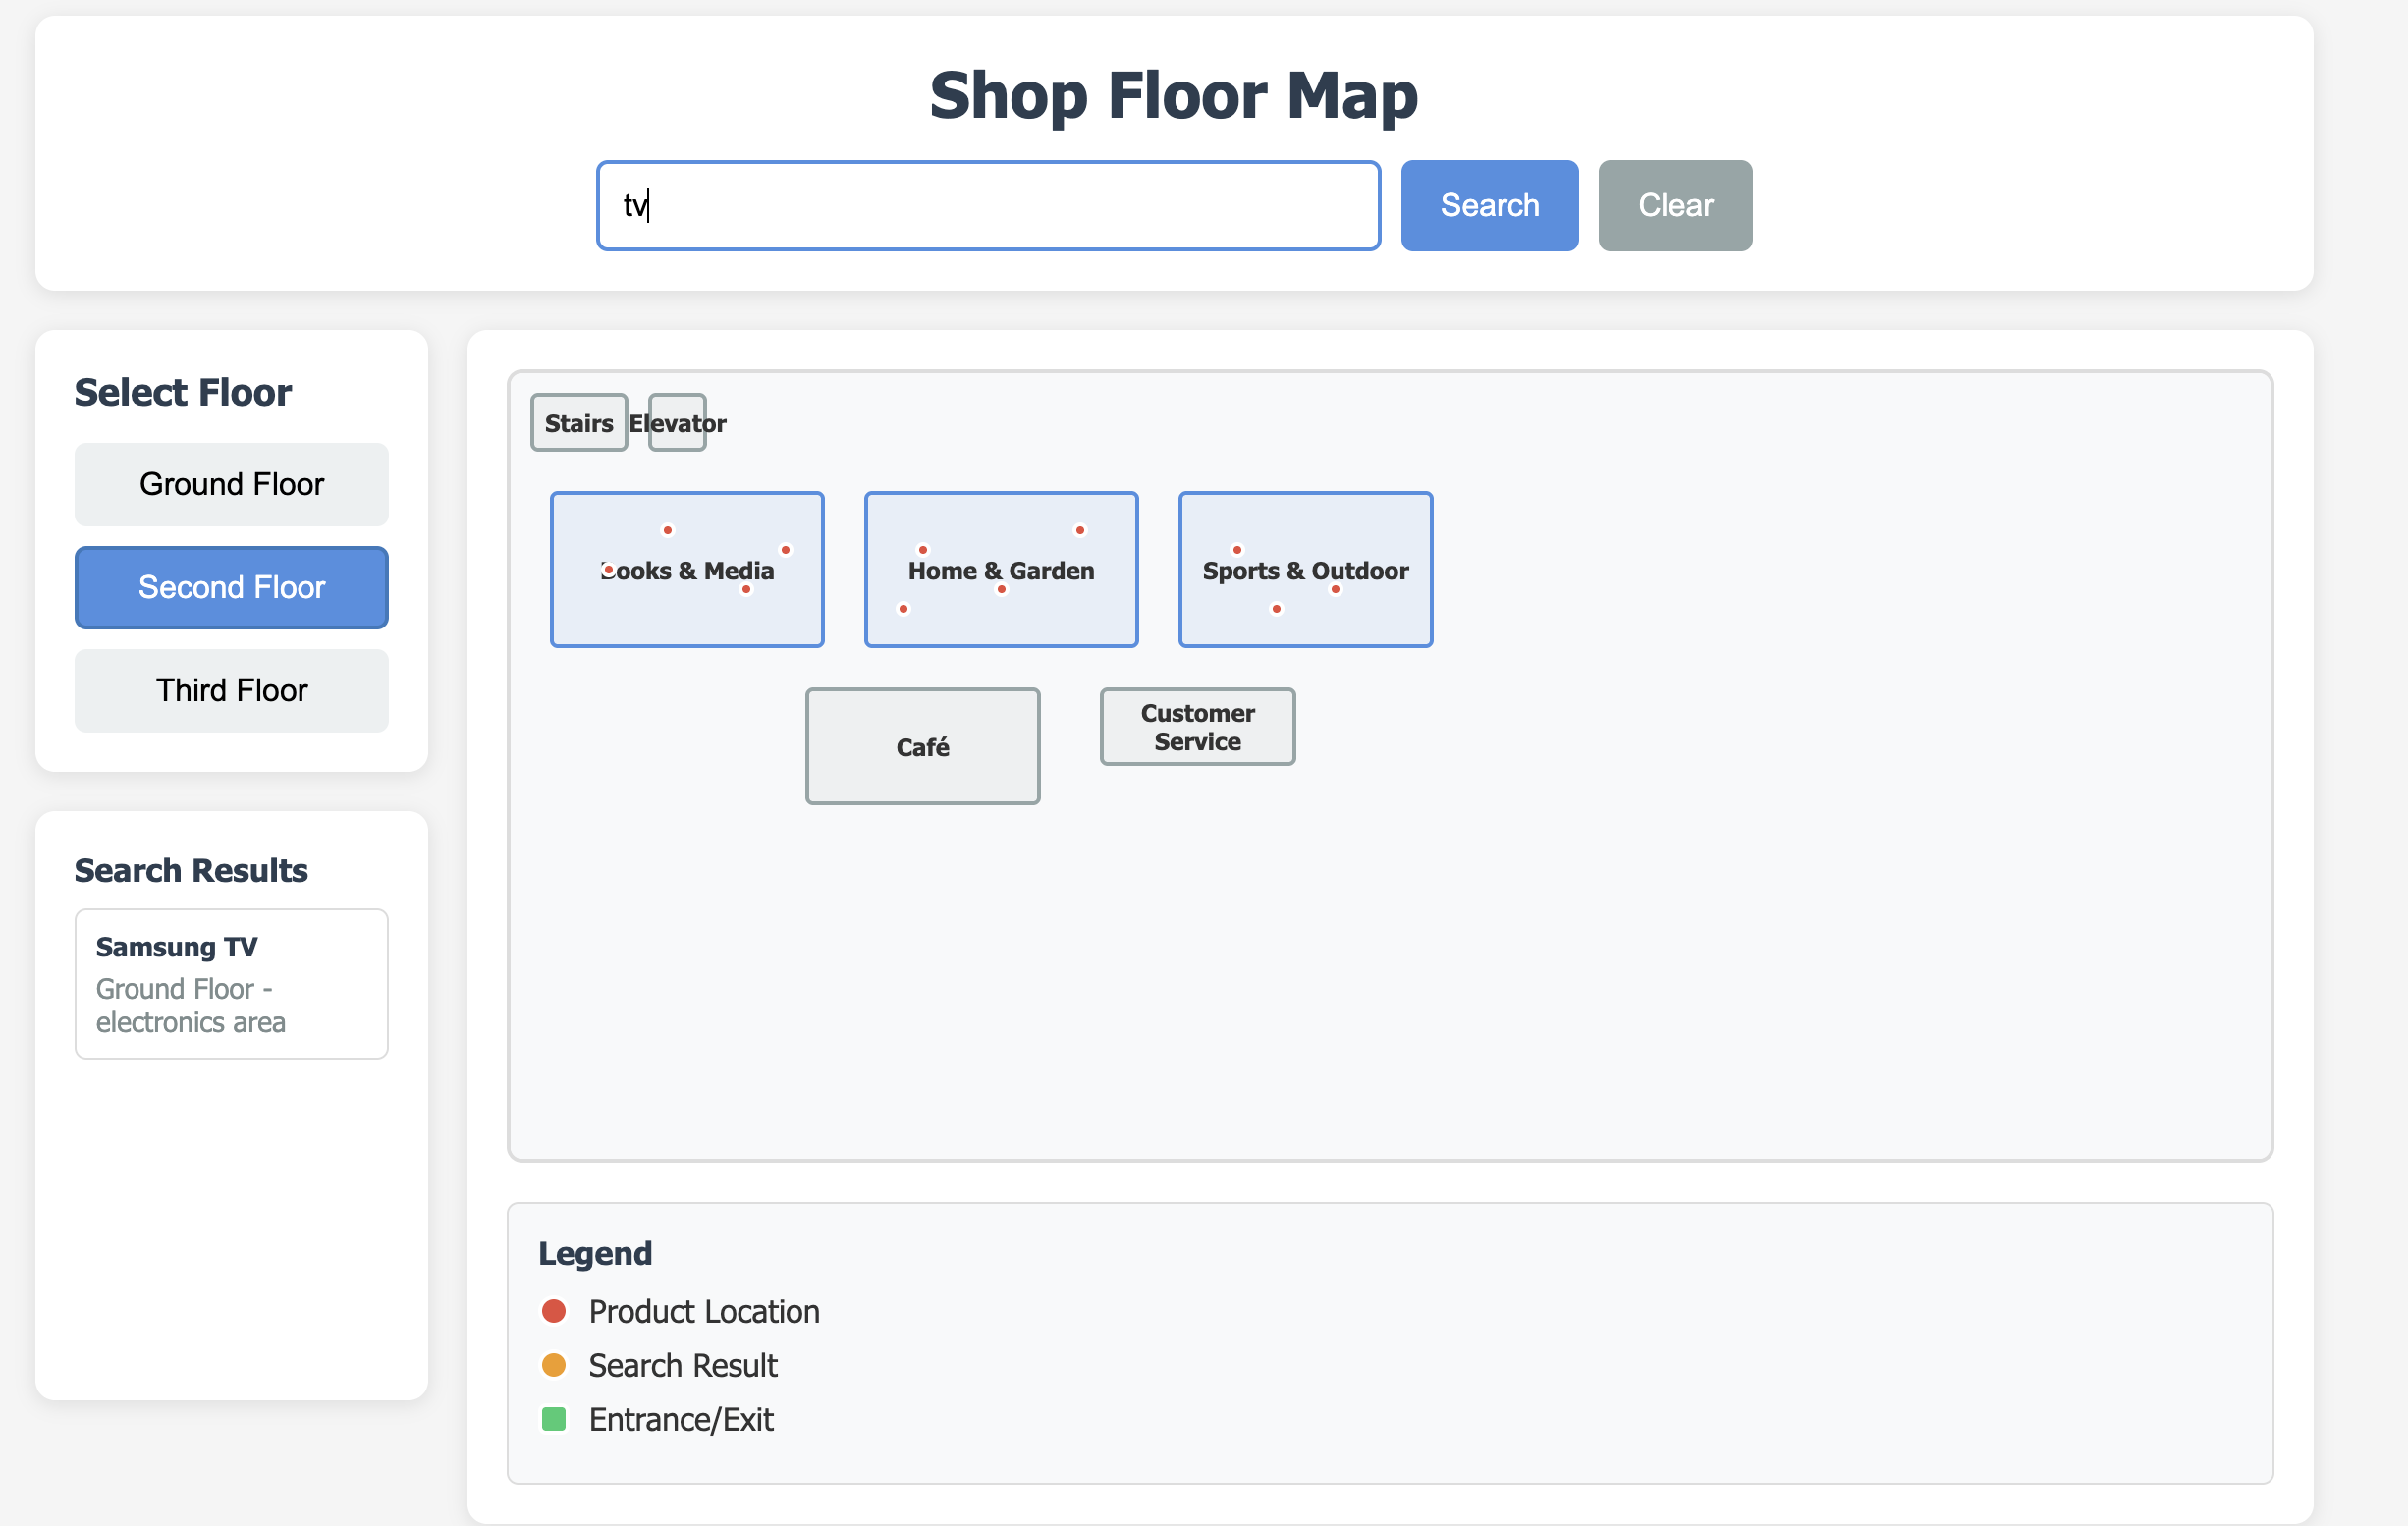
\includegraphics[width=0.7\linewidth]{figures/claude_cg_web.png}}
    \end{subcaptionbox}
    \caption{Claude Code-generated files: HTML, CSS, and JS for the shop map app}
    \label{fig:claude_code_output}
\end{figure}

\begin{figure}[htp]
    \centering
    \begin{subcaptionbox}[0.45\linewidth]{Gemini CLI Generation Output\label{fig:gemini_cg_output}}
        {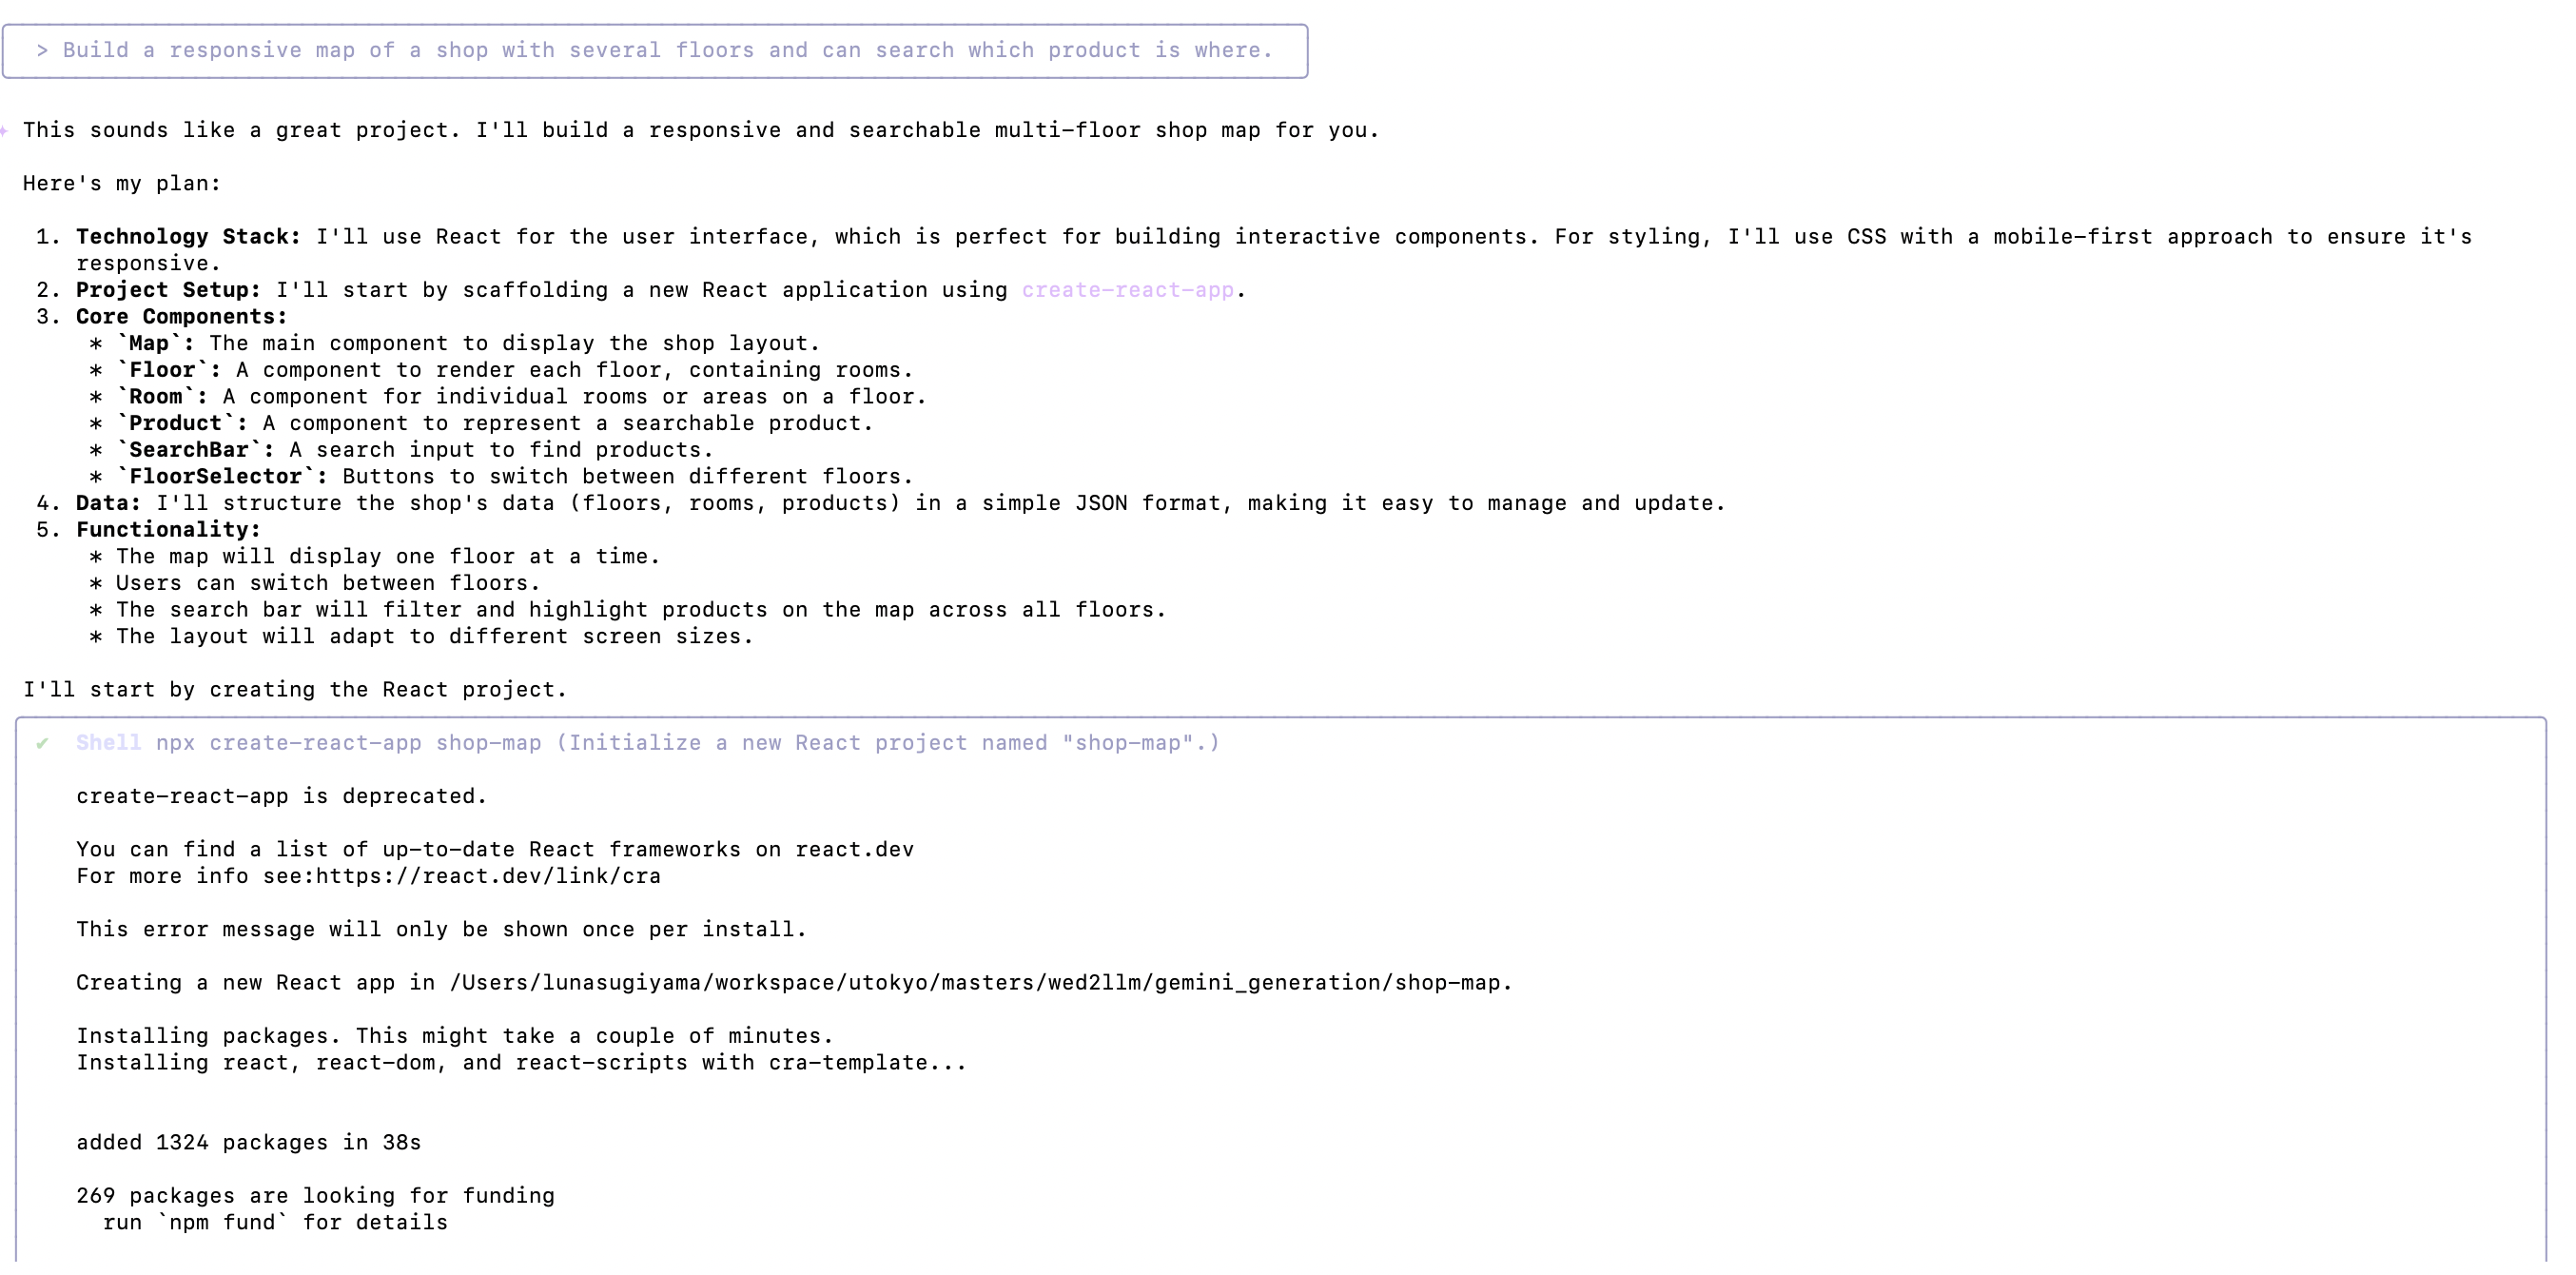
\includegraphics[width=\linewidth]{figures/gemini_cg_output.png}}
    \end{subcaptionbox}
    \hfill
    \begin{subcaptionbox}[0.45\linewidth]{Error in Gemini Generation\label{fig:gemini_cli}}
        {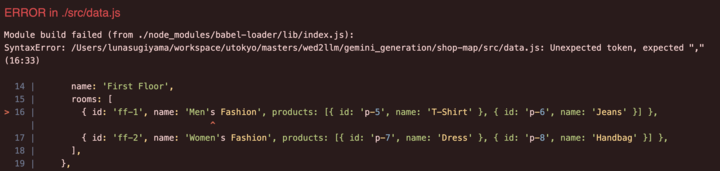
\includegraphics[width=\linewidth]{figures/gemini_cg_error.png}}
    \end{subcaptionbox}
    \begin{subcaptionbox}[0.45\linewidth]{Gemini CLI Generation Webpage\label{fig:gemini_cg_web}}
        {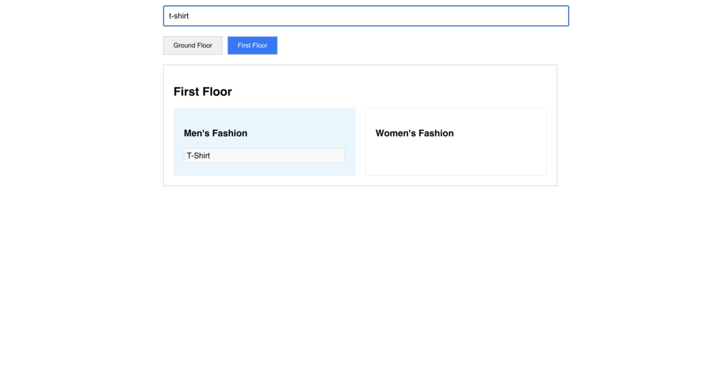
\includegraphics[width=\linewidth]{figures/gemini_cg_web.png}}
    \end{subcaptionbox}
    \caption{Gemini CLI-generated files: HTML, CSS, and JS for the shop map app}
    \label{fig:gemini_code_output}
\end{figure}

\section{Code Explanation Task Output}
\label{sec:code_explanation_output}
\subsection{Claude Code Output}
\begin{enumerate}
    \item Research PyTorch's loss.backward() implementation online
    \item Explain what loss.backward() does conceptually
    \item Detail the implementation mechanics and key components
\end{enumerate}
\subsection{Gemini CLI Output}
\begin{enumerate}
    \item First, I will start by searching for the string "backward" in the PyTorch repository to get a sense of the relevant files. 
    \item I'll focus the search on Python files to find the entry point, and then expand to C++ files.
    \item I'll also search for "autograd" as that's the relevant module.
\end{enumerate}
\bibliographystyle{plain}
\bibliography{references} % if you use a .bib file

\end{document}
